\chapter{Integration des Compilers}
\label{chap:compilerintegration}

In diesem Kapitel wird beschrieben, wie der Compiler in die Entwicklungsumgebung eingebunden wurde, um ein C-File nach Forth zu übersetzen und welche Möglichkeiten mit dem Eclipse-CDT für das Editieren von C-Files zur Verfügung stehen.

\section{Integration in Eclipse CDT}

Das Eclipse-CDT stellt Extension Points zur Verfügung, die gebraucht werden können um, einen Compiler zu integrieren. Diese Extension Points werden in den nächsten Kapiteln erläutert und es wird erklärt, wie der LCC dadurch in die Entwicklungsumgebung eingebunden wird.

\subsection{Configuration}
Eine Konfiguration wird verwendet, um verschiedene standard Tools und Options bereitzustellen, die ein Projekt auf eine bestimmte Weise kompilieren. Normalerweise existieren für ein Projekt zwei Konfigurationen, eine Debug- und eine Releasekonfiguration.\cite{managedbuildcdt}

\subsubsection{Verwendung}
Für die Entwicklungsumgebung existiert nur eine Konfiguration für den Release Build. Debug-spezifische Files werden vom Launch generiert.

\subsection{Tool}
Ein Tool definiert ein Programm, wie zum Beispiel einen Compiler oder Linker, welches vom Buildprozess verwendet wird.\cite{managedbuildcdt}

\subsubsection{Verwendung}
In der Entwicklungsumgebung wird nur ein Tool verwendet, das den LCC Compiler aufruft und somit das Forth File generiert. Für dieses Tool wurde eine Option (\verb!-S-Q!) definiert, welche den Peephole Optimizer des Compilers deaktiviert.

\subsection{Toolchain}
Eine Toolchain ist eine Liste von Tools, die gebraucht werden, um den Output des Projekts zu generieren.\cite{managedbuildcdt} 

\subsubsection{Verwendung}
Die von der Entwicklungsumgebung verwendete Toolchain beinhaltet nur das oben beschriebene Tool, um den LCC Compiler aufzurufen.

\subsection{CDT-Builder}
Der CDT-Builder repräsentiert das Werkzeug, welches verwendet wird um den Build-Prozess zu steuern. Typischerweise ist es eine Variante von \verb!make!.\cite{managedbuildcdt} 

\subsubsection{Verwendung}
Für die uCore-Entwicklungsumgebung wurde der Standard CDT-Builder verwendet. Zusätzlich werden die File-Endung der vom Compiler generierten Forth Files auf \verb!.fs! geändert.

\subsection{Project Builder}
Der Project Builder wird nicht vom Eclipse CDT, sondern vom normalen Eclipse Buildprozess zur Verfügung gestellt. Für die uCore Entwicklungsumgebung wird der Project Builder verwendet, um Fehler in den Umgebungsvariablen zu finden. Der Project Builder überprüft
%
\begin{itemize}
  \item ob das Programm \verb!lcc-mcore! im Pfad zu finden ist.
  \item ob eine Umgebungsvariable mit dem Namen \verb!GFORTHPATH! existiert.
  \item ob der letzte Pfad der Umgebungsvariable \verb!GFORTHPATH! zu einem gültigen Ordner zeigt
\end{itemize}
%
Falls einer dieser Schritte fehlschlägt, wird der Build-Vorgang abgebrochen und die Fehler werden in der Problem View von Eclipse angezeigt. Die Abbildung \ref{fig:patherror} zeigt die Eclipse Problem View mit einem Fehler im Pfad.

\begin{figure}[H]
	\centering
		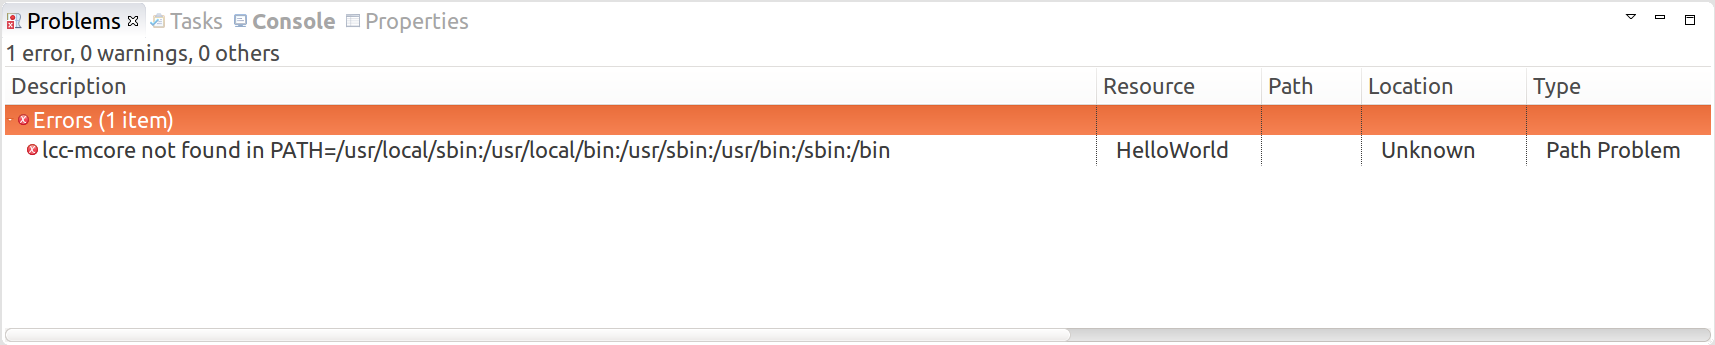
\includegraphics[scale=0.25]{compiler/patherror.png}
		\caption{Die Eclipse Problem View zeigt, dass das Program lcc-mcore nicht im Pfad gefunden wurde.}
		\captionsetup{margin=0cm,font={footnotesize}}
		\label{fig:patherror}
\end{figure}

In der Installationsanleitung im Anhang finden sich alle Schritte, die notwendig sind, um die Entwicklungsumgebung zu installieren.

